% IPEC2026.cls is based on IEEEtran.cls.
% Please read the instructions for IEEEtran.cls before using IPEC2026.cls.
\documentclass{IPEC2026}
\IEEEoverridecommandlockouts
% The preceding line is only needed to identify funding in the first footnote. If that is unneeded, please comment it out.
\usepackage{cite}
\usepackage{amsmath,amssymb,amsfonts}
\usepackage{algorithmic}
\usepackage{graphicx}
\usepackage{textcomp}
\usepackage{xcolor}
\usepackage{url} 
\def\BibTeX{{\rm B\kern-.05em{\sc i\kern-.025em b}\kern-.08em
    T\kern-.1667em\lower.7ex\hbox{E}\kern-.125emX}}
\begin{document}

\title{Real-Time DC-Link Capacitor Stress Reduction in Two-Level Three-Phase Inverters Using Adaptive Multi-Carrier PWM Method
\thanks{Research leading to these results has received funding from the EU CHIPSJoint Undertaking under grant agreement $n^o$ 101007326 (project PowerizeD) and from the (Swedish) partner national funding authority Vinnova. Funding for this research has also been received from the Swedish Energy Agency through the HEMIZERO project.}
}

% Please replace * with your track number
\track{: 4 Motor Drive and Control}

\maketitle

\begin{abstract}
This paper presents a novel multi-carrier pulse width modulation (PWM) technique for two-level three-phase inverters to reduce the current stress of the DC-link capacitors, thereby improving system reliability and extending capacitor lifetime. 
Unlike conventional interleaving approaches used in parallel inverter systems or pulse synchronization in multi-stage converters, the proposed method applies adaptive interleaving between the inverter legs of a single two-level three-phase inverter unit.
The carrier phase shifts are dynamically updated in each control cycle based on real-time duty cycles and leg currents, enabling effective redistribution of switching events and minimizing capacitor RMS current. 
%To overcome the implementation complexity associated with high-dimensional input spaces, the method leverages the symmetry and balance of three-phase systems to reduce the number of independent variables. 
%This allows for the creation of a compact look-up table through normalization and transformation, enabling efficient real-time operation.
Analytical results confirm the effectiveness of the proposed PWM strategy in significantly reducing ripple current up to 27\%  and enhancing the reliability and lifetime of the DC-link capacitors. \color{red} The experimental validation will be made for different operating points of the inverter. \color{black}

\end{abstract}

\begin{IEEEkeywords}
 Motor drive, DC-link current ripple, sinusoidal pulse width modulation, multi-carrier PWM, voltage source inverter.
\end{IEEEkeywords}


\section{Introduction}
\label{sec:introduction}
%\PARstart{T}{wo-level}
Two-level three-phase voltage source inverters (VSIs)  have still remained as one of the dominant topologies in industrial motor drives thanks to their reduced component count, simplicity, ease of control, and cost-effectiveness~\cite{IndustrialMotorDrives,IndustrialDrives}.
Despite these advantages, reliability concerns continue to pose a significant challenge.
One of the main reliability concerns is caused by DC-link capacitors, reportedly responsible for approximately 30\% of industrial power converter failures~\cite{CapacitorFailure}. 
A key contributor to these failures is the ripple current flowing through the capacitor, which induces thermal stress and accelerates aging, thereby reducing its operational lifetime \cite{LifetimeExtension-SingleInverter-PWM, LifeTimeExtension-ThreeLevel-CarrierBased}.
Accordingly, various techniques have been investigated to reduce the ripple current magnitude and spectral content to enhance the reliability and enhance the lifetime of the DC-link capacitors \cite{PWM_methods1, SectorBased-PWM, DualMotor-modulation1,multiinverter-modulation1, dualmotor-interleaving, Interleaving-DualMotor, DualMotor-Interleaved-Parallel, PWM-CarrierBased, TwoStage-RippleReduction,  PhaseShift-PreConverter, DiscontinousPWM-ThreeLevel, VariableSwitchingSequence-ThreeLevel, Three-level-Phase-Disposition, AdaptiveSwitching-solarInverter, RippleReduction-4-Wires}.

Among the various ripple reduction strategies, interleaving in multi-inverter systems has demonstrated promising results \cite{DualMotor-Interleaved-Parallel,multiinverter-modulation1,dualmotor-interleaving, DualMotor-modulation1,Interleaving-DualMotor}.
Several studies show that optimal phase shifting and current ripple synchronization among parallel inverters or multiphase machines effectively reduce DC-link ripple and enhance capacitor longevity.
Similarly, in two-stage inverter systems, ripple mitigation has been achieved through dynamic coordination of switching sequences between the front-end and inverter stages
using interleaved carriers \cite{PhaseShift-PreConverter, TwoStage-RippleReduction}.

In contrast to these approaches, which rely on multiple inverter legs or cascaded stages, this paper proposes a novel modulation strategy that applies adaptive interleaving between legs of a single two-level three-phase VSI.
In the proposed method, leg-specific carrier phase shifts are dynamically updated in each control cycle based on the instantaneous duty ratios and phase currents.
This real-time adaptation redistributes the switching instants to minimize the total RMS current stress on the DC-link capacitor, thereby enhancing its lifetime.
Notably, this strategy requires no additional hardware, such as parallel inverters or a front-end converter, making it a practical and low-complexity solution for ripple reduction.
While the concept builds on interleaving principles, implementing it within a single inverter introduces new challenges due to the time-varying nature of phase currents and the interaction of three duty ratios and three leg currents. That is to say, determining the optimal carrier phase shifts in real time is computationally intensive due to the high dimensionality of the problem.
Therefore, the paper introduces a look-up table (LUT) that is constructed offline to estimate the carrier phase shifts regarding the duty ratios and leg currents covering all the possible operating points of the inverter. 
The comparison of the proposed method with existing literature is summarized in Table~\ref{tab:ripple_comparison}. 
Unlike prior approaches that rely on parallel inverters, multiphase drives, or additional DC–DC stages, the proposed method achieves effective ripple reduction within a single two-level three-phase VSI. 
It requires no extra hardware, with the only limitation being the need for an offline look-up table (LUT) to enable adaptive carrier phase shifting in real time.


\begin{table*}[t]
\centering
\caption{DC-Link Capacitor Ripple Reduction Strategies in Literature}
\label{tab:ripple_comparison}
\begin{tabular}{p{1.2cm} p{3.5cm} p{3.8cm} p{8cm}}
\hline
Ref. & Topology & Approach & Evaluation \\
\hline
\cite{Interleaving-DualMotor} & Integrated modular drive & Multi-phase interleaving & Requires multi-phase IMMD; Applying constant carrier phase shifts \\
\cite{DualMotor-Interleaved-Parallel} & Two parallel 2L VSIs & Hybrid carrier-based PWM & Needs two inverters; Updating reference signals  \\
\cite{TwoStage-RippleReduction} & Single-phase 2-stage inverter & Carrier shaping in DC-DC stage & Needs pre-stage converter; Altering carrier signals  \\
\cite{PhaseShift-PreConverter} & Three-phase 2-stage inverter & Generalized carrier-shift method & Needs pre-stage converter;  Altering carrier signals \\
This work & Single 2L-3Ph VSI & Real-time multi-carrier PWM & No extra hardware; Applying adaptive carrier phase shifts\\
\hline
\end{tabular}
\end{table*}




% Constructing a direct look-up table (LUT) for all possible input combinations is infeasible.
% To overcome this, the method leverages the symmetry and balance properties of the three-phase system to reduce the number of independent variables.
% Through appropriate normalization and transformation, the input space is compacted, enabling the construction of a computationally efficient LUT suitable for real-time implementation.


The remainder of this paper is organized as follows.
% Section~II presents a lifetime estimation model for DC-link capacitors under ripple-induced thermal stress. 
Section~II analyzes the capacitor current behavior in a two-level three-phase voltage source inverter and provides a mathematical formulation for RMS stress evaluation. 
The conventional single-carrier PWM method is reviewed in Section~III, while the proposed multi-carrier PWM technique is detailed in Section~IV. 
%Section~VI presents simulation results demonstrating the effectiveness of the proposed approach. 
Section~V presents the comparison of the conventional method and proposed method. 
Section~VI discusses implementation aspects, including lookup table construction. Experimental validation of the technique is provided in Section~VII. 
Finally, the conclusion is drawn in Section~VIII.

%\section{DC-Link Capacitor Lifetime Estimation}
%\label{sec:Capacitor Lifetime Analysis}
%The lifetime of DC-link capacitors depends on several stress factors, including voltage, current, temperature, and humidity.
%In this study, a simplified lifetime model commonly used in the literature~\cite{DPWM-TwoLevel} is employed to estimate capacitor degradation, and is given by
%\begin{equation}
%    L= L_{nom} \times (\frac{V_{op}}{V_{nom}})^{n}  \times 2^{\frac{T_0^{hot}-T^{hot}}{10}}
%\end{equation}
% where $L$ is the predicted lifetime, $L_0$ is the lifetime under test conditions, $V_{op}$ is the operating voltage, $V_{nom}$ is the rated voltage, $T^{hot}$ is the operating hotspot temperature, $T_0^{hot}$ is the allowable hotspot temperature under a test condition, and $n$ is the voltage stress coefficient \cite{PhaseShift-PreConverter}. 
% As shown, the model links thermal stress to lifetime reduction, with temperature rise primarily caused by internal power losses. This temperature can be modeled as
% \begin{equation}
% T^{hot}= T_{ambient}+ R_{eq} \times P_{Loss-ESR}
% \end{equation}
% where $T_{ambient}$ is the ambient temperature, $R_{t}$ is the equivalent thermal resistance, and $P_{Loss-ESR}$ represents power losses due to the capacitors'  equivalent series resistance (ESR). 
% These losses mainly result from the ripple current flowing through the ESR, and can be  calculated as
% \begin{equation}
%     P_{loss-ESR}= \sum_{n=1}^{\infty} \bigg( I_{RMS}^2(f_n) \times ESR(f_n) \bigg)
% \end{equation}
% where $I_{RMS}(f_n)$ is the DC-link current RMS at the frequency of $f_n$, and $ESR(f_n)$ is the equivalent series resistance of the capacitors at that frequency.
% It is also important to note that, as the capacitor ages, its ESR tends to increase due to wear-out mechanisms, which further amplifies the effect of ripple current on thermal stress and accelerates the degradation process ~\cite{CapacitorLifeTime-3LANPNC-Sector}.
\section{DC-Link Current Analysis of the Inverter}
\label{sec:SystemStructure}
Fig.~\ref{fig:system_structure} illustrates a conventional two-level three-phase (2L-3Ph) voltage source inverter (VSI) along with its simplified equivalent circuit. 
\vspace{-4mm}
\begin{figure}[h!]
    \centering
    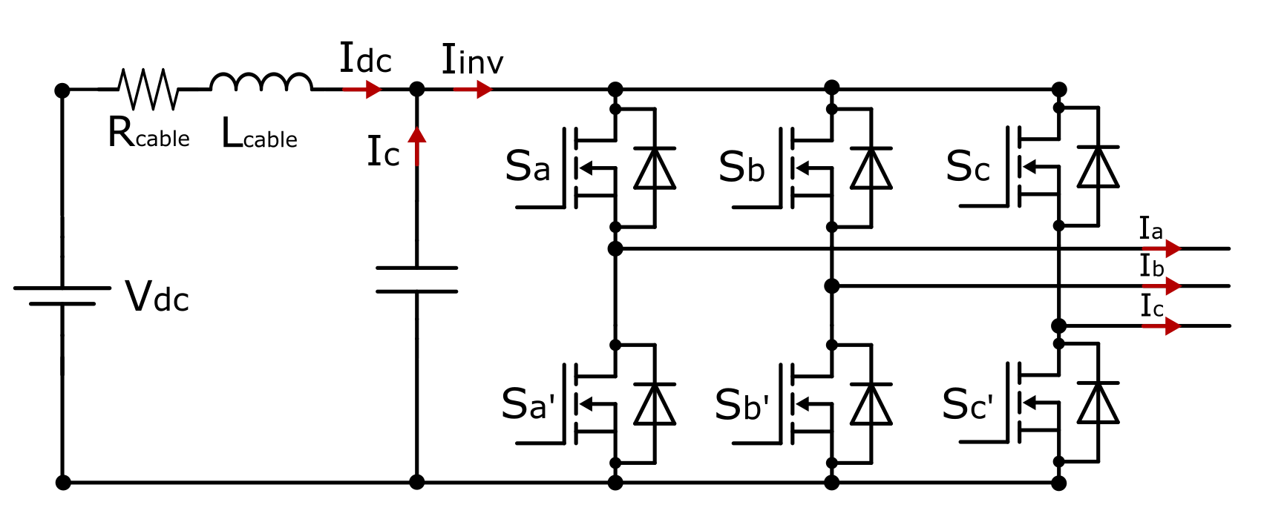
\includegraphics[width=1\linewidth]{A-Figures/Intro-DCLinkModelling/TwoLevelInverter.png}
     \vspace{-7mm}
    \caption{Two-level three-phase voltage source inverter.}
    \label{fig:system_structure}
\end{figure}
\vspace{-2mm}

The equivalent model highlights the DC-link current path, under the assumption that all high-frequency components generated by inverter switching are fully absorbed by the DC-link capacitor.
Therefore, mathematically, the instantaneous capacitor current [$i_{cap}(t)$] can be expressed as the sum of individual phase currents [$i_x(t)$ for $x\in\{a,b,c\}$] multiplied by their respective switching functions [$S_x(t)$ for $x\in\{a,b,c\}$], minus the average DC component [$\overline{i}_{dc}$] as given by
\begin{equation}
    i_{cap}(t) = \sum_{x\in\{a,b,c\}} i_x(t)S_x(t) - \overline{i}_{dc}.
\end{equation}
The switching function for each phase is determined by comparing the phase reference voltage as 
\begin{equation}
    v_{x,ref}(t) = m_a\cos(\theta(t) - 2\pi(x-1)/3),
\end{equation}
with the triangular carrier waveform as
\begin{equation}
\text{tri}(2\pi f_{sw}t-\theta_{x,carrier}),
\end{equation}
and can be calculated as 
\begin{equation}
\begin{aligned}
S_x^{conv}(t) &= 
\begin{cases} 
1 & \text{if } v_{x,ref}(t) > \text{tri}(2\pi f_{sw}t-\theta_{x,carrier}), \\
0 & \text{otherwise},
\end{cases}
\end{aligned}
\end{equation}
where $m_a$ is the modulation index, $f_{sw}$ is the switching frequency, $\theta_{x,carrier}$ is the carrier phase of legs for $x\in\{a,b,c\}$. 


In this paper, a hierarchical approach, covering both switching-period and fundamental-period dynamics of inverter operation, is proposed to analyse the DC-link current. 
First, at the switching period ($T_{sw} = 1/f_{sw}$), the instantaneous RMS current is computed as:
\begin{equation}
I_{cap,rms}[k] = \sqrt{\frac{1}{T_{sw}}\int_{(k-1)T_{sw}}^{kT_{sw}} i_{cap}^2(t) dt}\quad \text{for } k = 1,2,...,N_{sw}
\end{equation}
where $N_{sw} = f_{sw}/f_1$ is the number of switching intervals within one fundamental period.
During this period, both the reference voltages and phase currents are assumed to vary slowly as the switching frequency is much faster than the fundamental frequency, as given:
\begin{equation}
\begin{aligned}
&v_{x,ref}[k] \approx m_a\cos\left(\frac{2\pi k}{N_{sw}} + \theta_{fund} - \frac{2\pi(x-1)}{3}\right) \\
&i_x[k] \approx I_{pp}\cos\left(\frac{2\pi k}{N_{sw}} + \theta_{fund} - \frac{2\pi(x-1)}{3} - \theta_{phase-angle}\right)
\end{aligned}
\end{equation}
which allows the capacitor current waveform to be evaluated at quasi-static conditions within each switching cycle.
Then, the steady-state fundamental-period RMS current can be calculated by combining all switching-period RMS, as given by:

\begin{equation}
I_{cap,rms}^{total} = \sqrt{\frac{1}{N_{sw}}\sum_{k=1}^{N_{sw}} I_{cap,rms}^2[k]}
\end{equation}

This formulation shows that minimizing each $I_{c,rms}[k]$ directly reduces $I_{c,rms}^{total}$, which means that individual minimization during each switching interval leads to fundamental-RMS minimization.


\section{Conventional Single-Carrier-Based PWM}
The conventional single-carrier-based PWM scheme employs identical triangular carrier signals for all three phases, given in Fig. \ref{fig:ConventionalPWM}. 
The conventional method's performance is fundamentally constrained by the uncontrolled switching events, which prevent the optimum harmonic cancellation between phases regarding each switching interval.
An example operation, the key waveforms are given as shown in Fig. \ref{fig:keywaveforms_conventional}. 

\begin{figure}[h!]
    \centering
    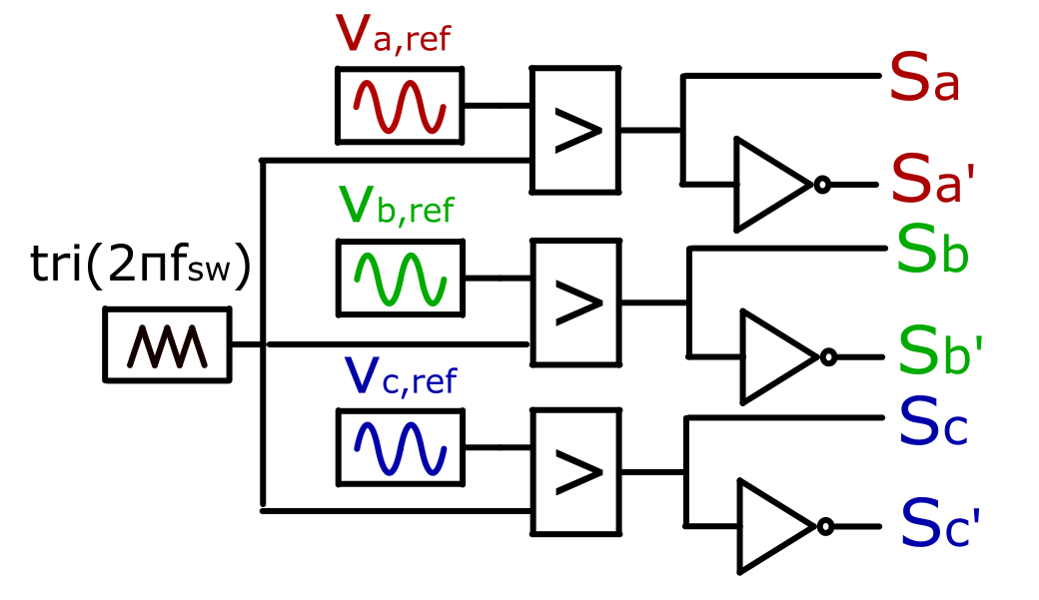
\includegraphics[width=0.7\linewidth]{A-Figures/Intro-DCLinkModelling/conventionalPWM.png}
     \vspace{-3mm}
    \caption{Conventional Single-Carrier PWM}
    \label{fig:ConventionalPWM}
\end{figure}
\begin{figure}[h!]
    \centering
    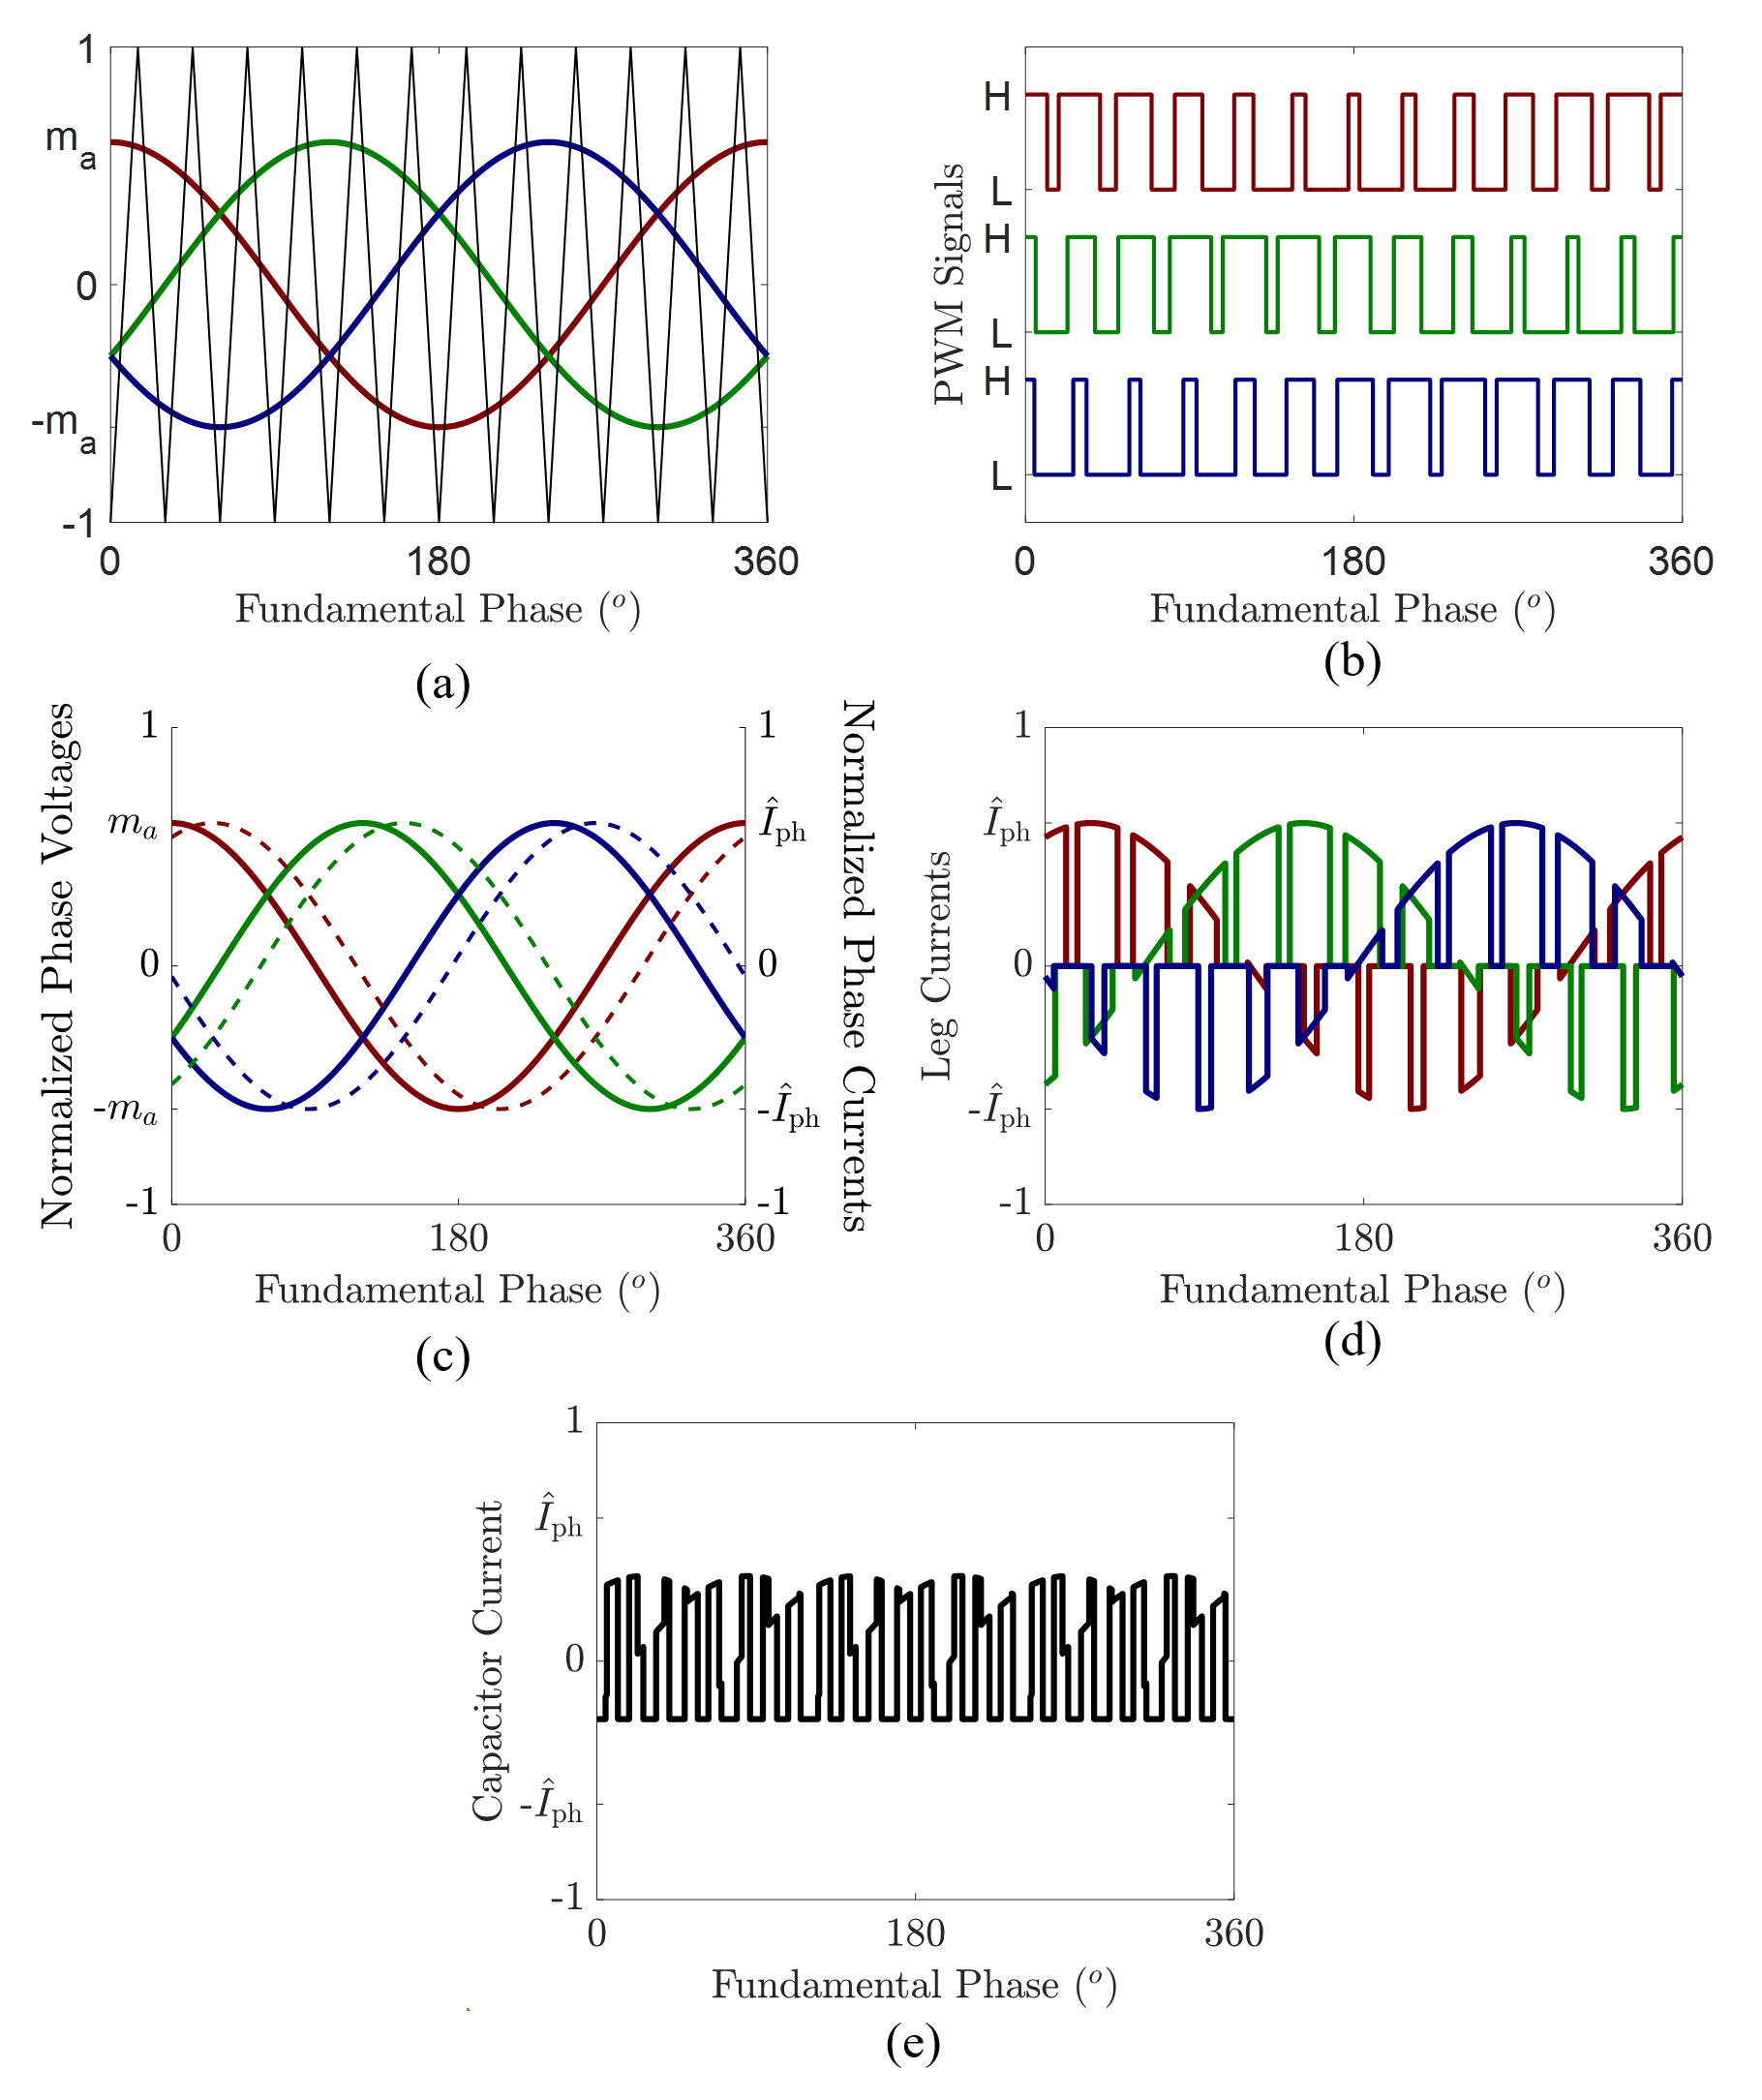
\includegraphics[width=1\linewidth]{A-Figures/Modulations/KeyWaveformsconvenitonal.png}
    \vspace{-8mm}
    \caption{Key waveforms in conventional SPWM. Red, green, and blue curves correspond to phases A, B, and C, respectively. (a) Reference signals and common triangular carrier waveform. (b) Resulting PWM gate signals for each inverter leg. (c) Normalized phase voltages (solid) and phase currents (dashed). (d) Leg currents. (e) DC-link capacitor current waveform.}
    \label{fig:keywaveforms_conventional}
\end{figure}


\newpage
\section{Proposed Multi-Carrier PWM Technique}
The proposed method introduces an adaptive interleaving by applying phase-shifted triangular carrier signals, which is updated within each switching period,  to each leg of a two-level three-phase inverter, as the proposed PWM scheme is shown in Fig. \ref{fig:proposedPWM}. 

\begin{figure}[h!]
    \centering
    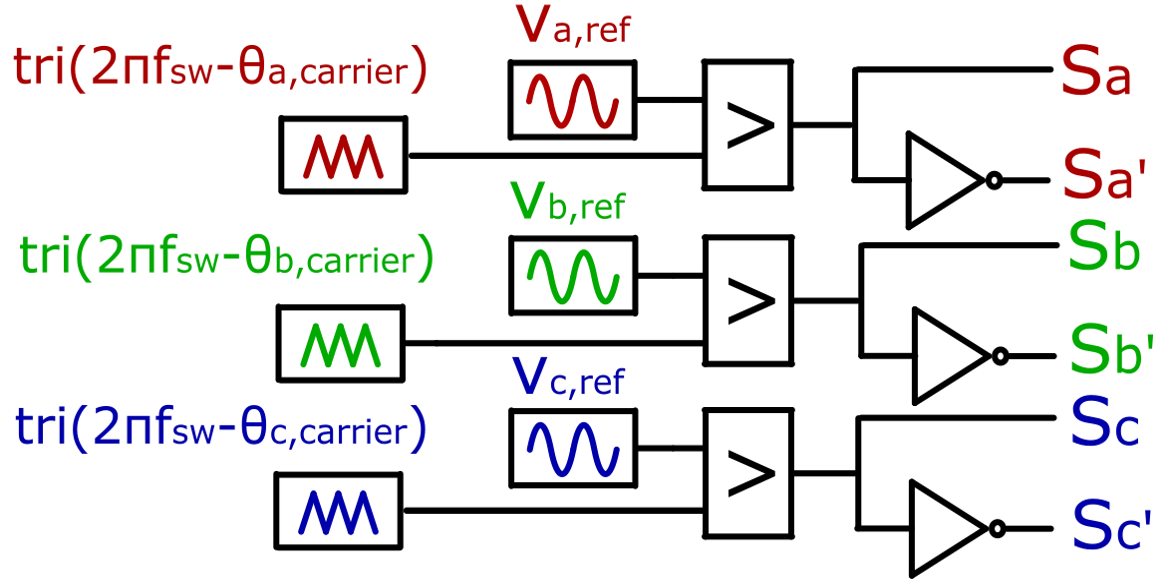
\includegraphics[width=0.8\linewidth]{A-Figures/Intro-DCLinkModelling/proposedPWM.png}
    \vspace{-3mm}
    \caption{Proposed Multi-Carrier PWM}
    \label{fig:proposedPWM}
\end{figure}

Each phase is assigned an individual carrier waveform with a phase displacement \( \delta_x \) (\( x \in \{a,b,c\} \) ), where \( \delta_a = 0 \), \( \theta_{b,\mathrm{carrier}} \), and \( \delta_c = \theta_{c,\mathrm{carrier}} \). An example operation, the key waveforms are  given as shown in Fig. \ref{fig:keywaveforms_proposed}. 

\begin{figure}[h!]
    \centering
    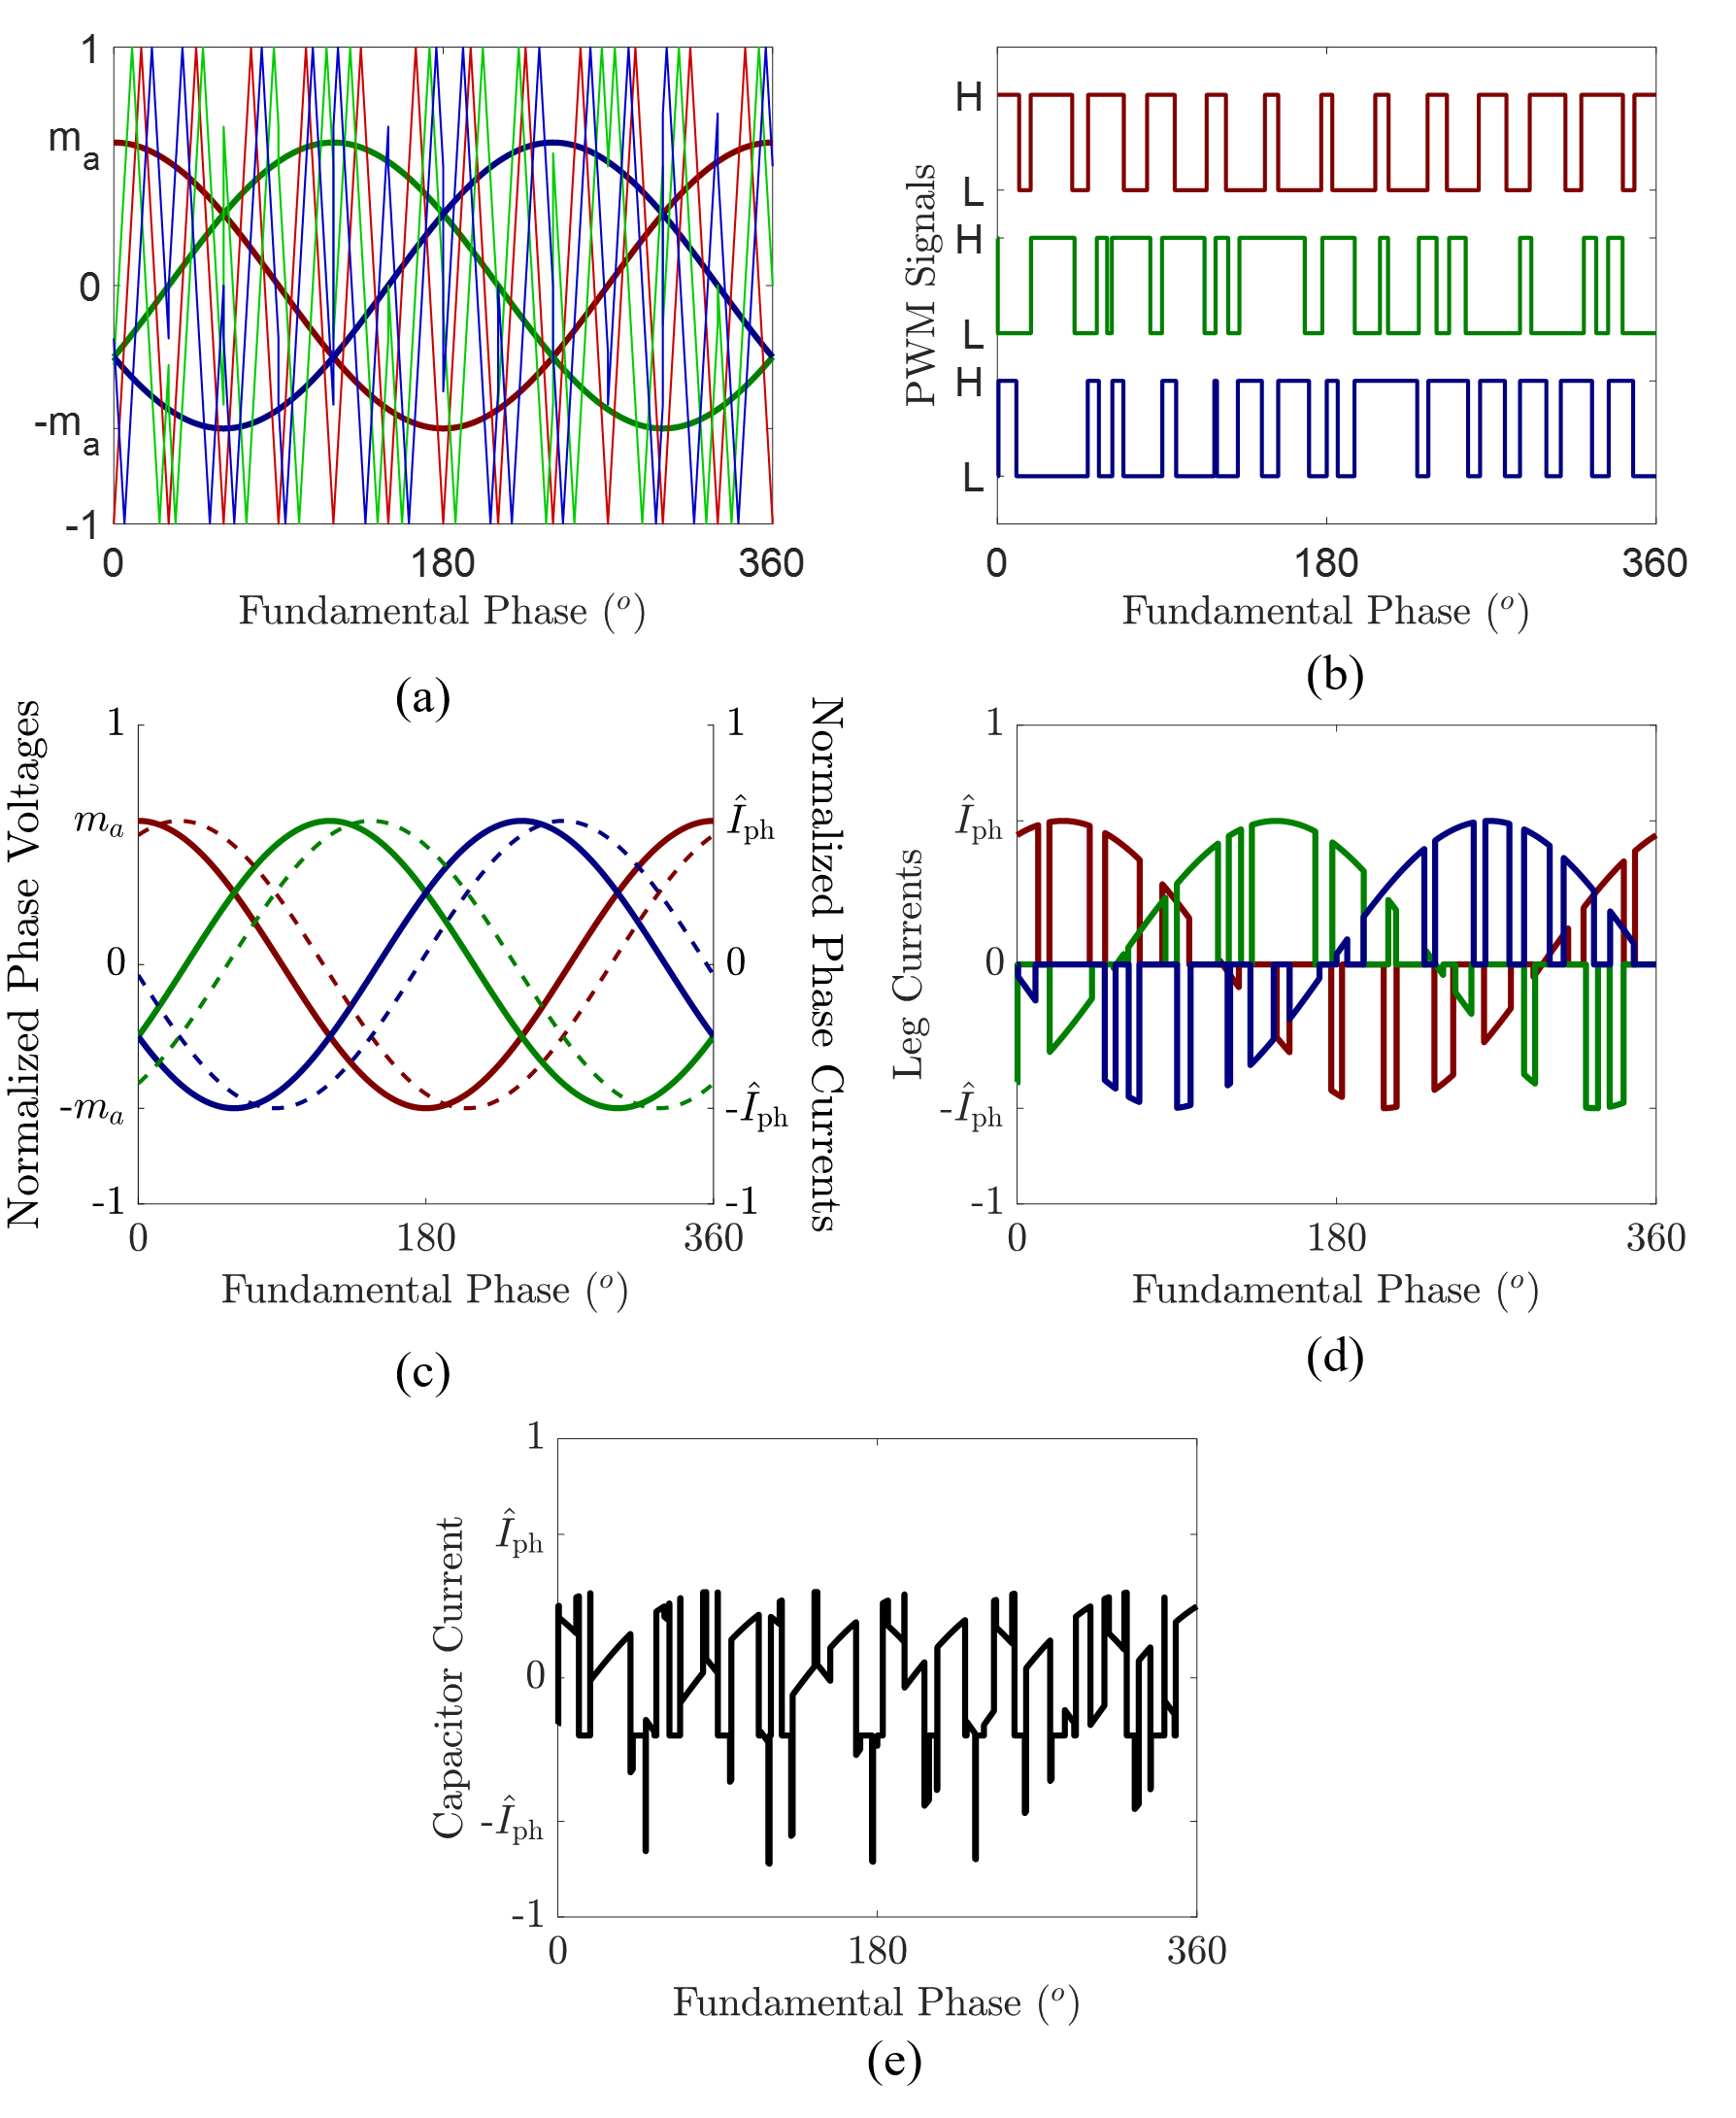
\includegraphics[width=1\linewidth]{A-Figures/Modulations/KeyWaveformsProposed.png}
     \vspace{-8mm}
    \caption{Key waveforms in the proposed multi SPWM. Red, green, and blue curves correspond to phases A, B, and C, respectively. (a) Reference signals and common triangular carrier waveform. (b) Resulting PWM gate signals for each inverter leg. (c) Normalized phase voltages (solid) and phase currents (dashed). (d) Leg currents. (e) DC-link capacitor current waveform.}
    \label{fig:keywaveforms_proposed}
\end{figure}

The goal is to dynamically determine the optimal phase shifts \( \theta_{b,carrier}^{opt} \) and \( \theta_{c,carrier}^{opt} \) in each switching cycle to minimize the RMS current through the DC-link capacitor.
The optimal phase shifts \( (\theta_{b,carrier}^{opt}, \theta_{c,carrier}^{opt}) \) are obtained by minimizing the capacitor RMS current over the switching period as 
\begin{equation}
(\theta_{b,carrier}^{opt}[k], \theta_{c,carrier}^{opt}[k]) = \arg\min_{\theta_b, \theta_c} \left( \int_{(k-1)T_{sw}}^{kT_{sw}} i_{cap}^2(t) \, dt \right)
\end{equation}
The optimization is done offline with respect to distinct duty ratios and phase current values, then it is implemented in the controller, which will be discussed in the following sections. 

% Therefore, the control algorithm can be created as shown in Fig. To estimate the minimum value, we need to get current measurement feedbacks, bla bla...


\section{Performance Assessment of the Proposed Multicarrier PWM Method}
In this section, the effectiveness of the proposed multicarrier PWM method is evaluated in terms of reducing the RMS current stress on the DC-link capacitor. 
The assessment is conducted through numerical calculations. 
Two distinct operating points are selected for both the conventional and the proposed systems, and the corresponding RMS values of the capacitor current at the switching frequency are calculated. The comparison results are presented in Fig.~\ref{fig:RMS_comparison_switching}.

\begin{figure}[h!]
    \centering
    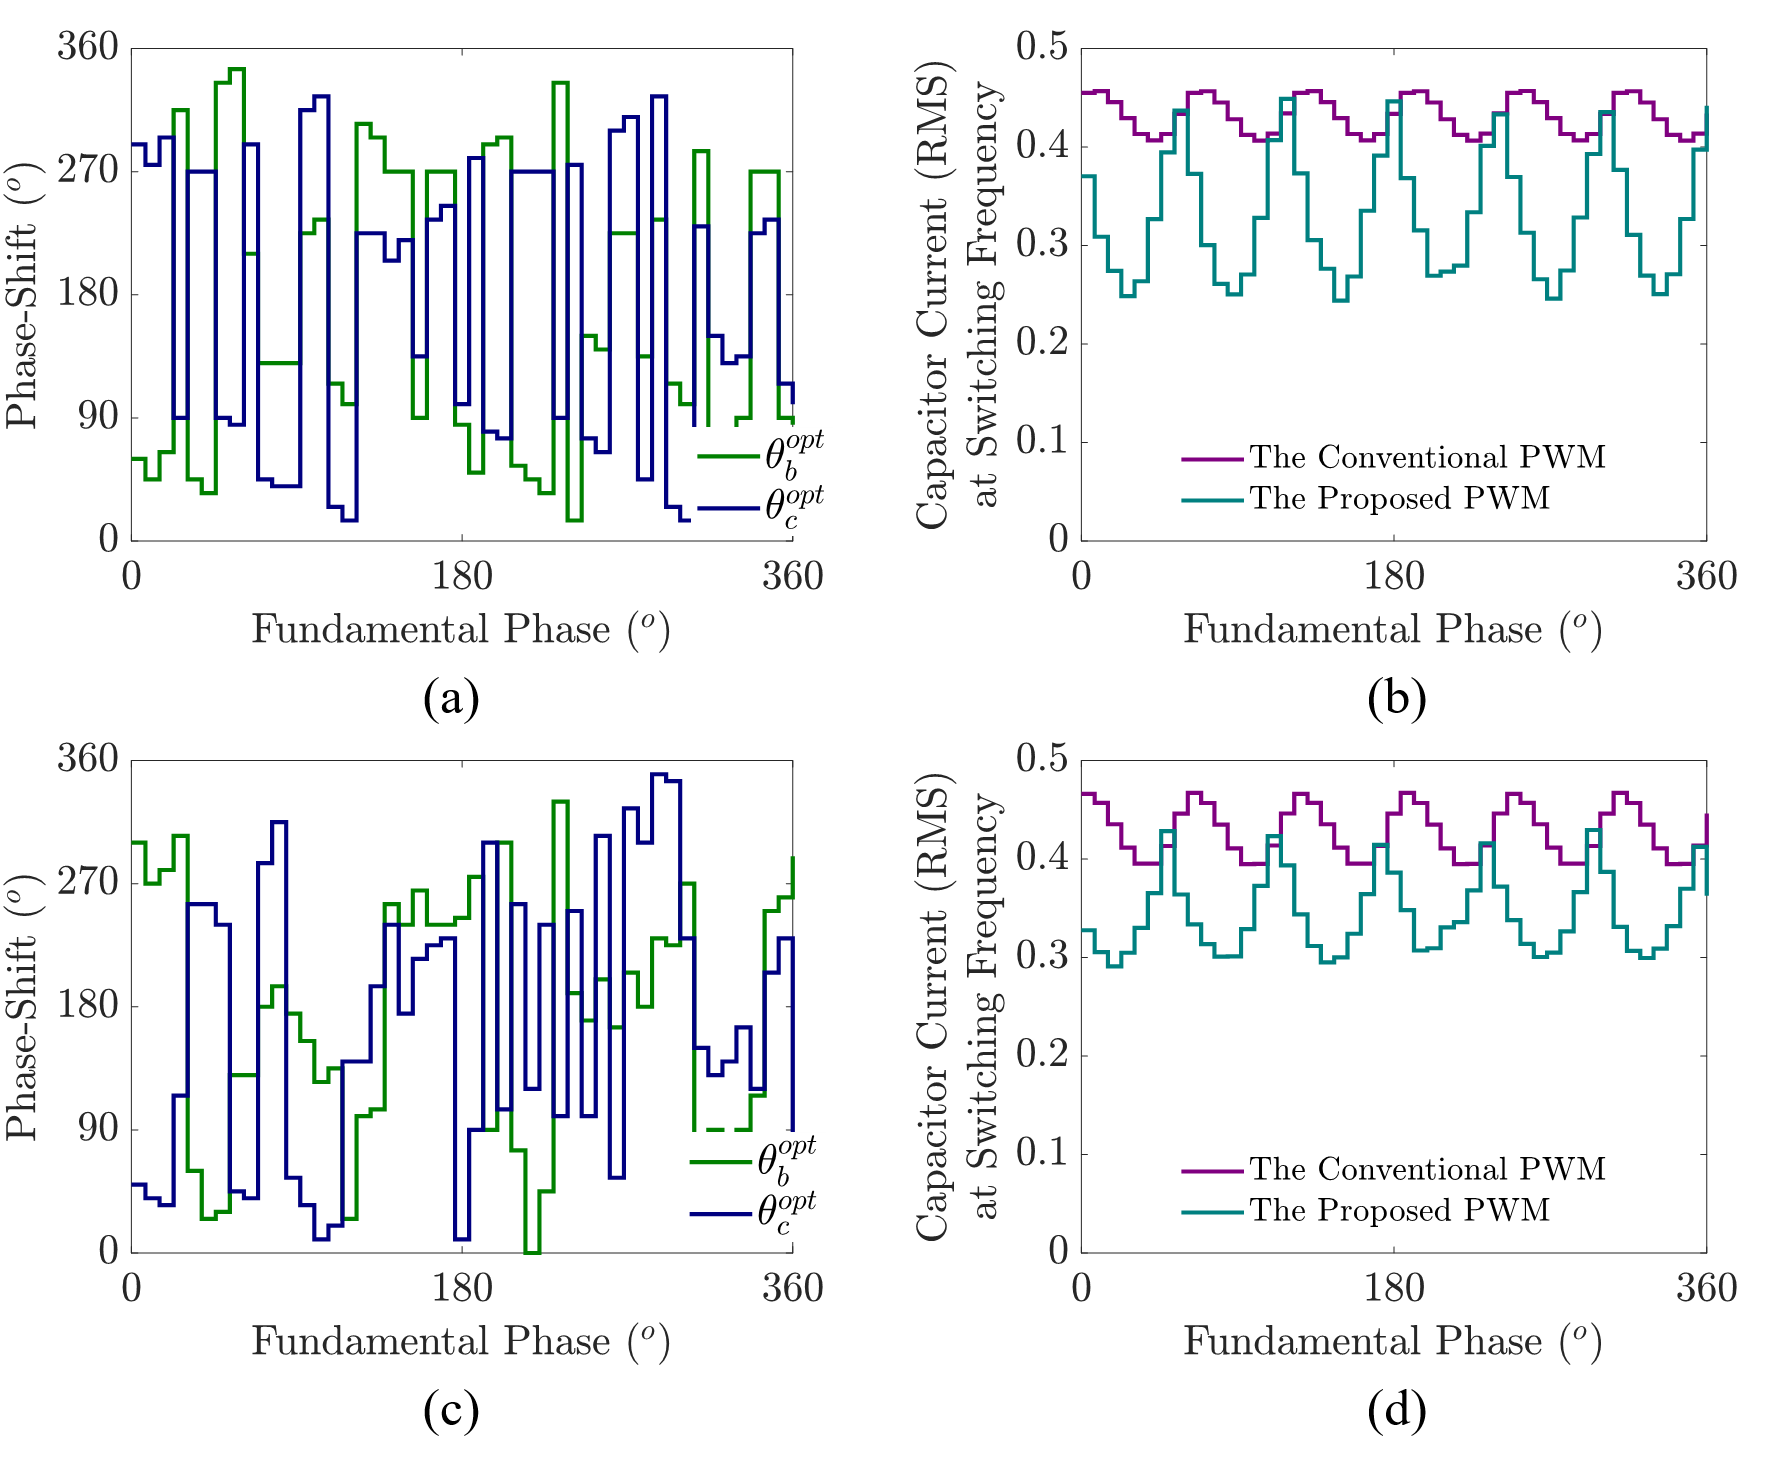
\includegraphics[width=1\linewidth]{A-Figures/Simulation/RMSComparison.png}
    \vspace{-8mm}
    \caption{Capacitor current analysis under various modulation conditions. (a) Optimum carrier phase shift for \( m_a = 0.6 \), \( I_{\text{ph}} = 1~\text{p.u.} \), and power factor \( p.f = 0.9 \). (b) RMS capacitor current at the switching frequency for the same condition. (c) Optimum carrier phase shift for \( m_a = 0.8 \), \( I_{\text{ph}} = 1~\text{p.u.} \), and power factor \( p.f = 0.95 \). (d) RMS capacitor current at the switching frequency comparison for the same condition.}
    \label{fig:RMS_comparison_switching}
\end{figure}


Then, Fig.~\ref{fig:rms_results_tot} illustrates the root mean square (RMS) value of the DC-link capacitor current as a function of the modulation index (\( m_a \)) and power factor (\( p.f. \)), comparing the conventional single-carrier PWM with the proposed multicarrier modulation strategy.
These results indicate that the proposed method achieves a notable reduction in RMS current (up to \%27) across a wide range of operating conditions.
This reduction leads to decreased thermal stress on the capacitor, which in turn contributes to an extended capacitor lifetime.

\begin{figure}[h!]
    \centering
    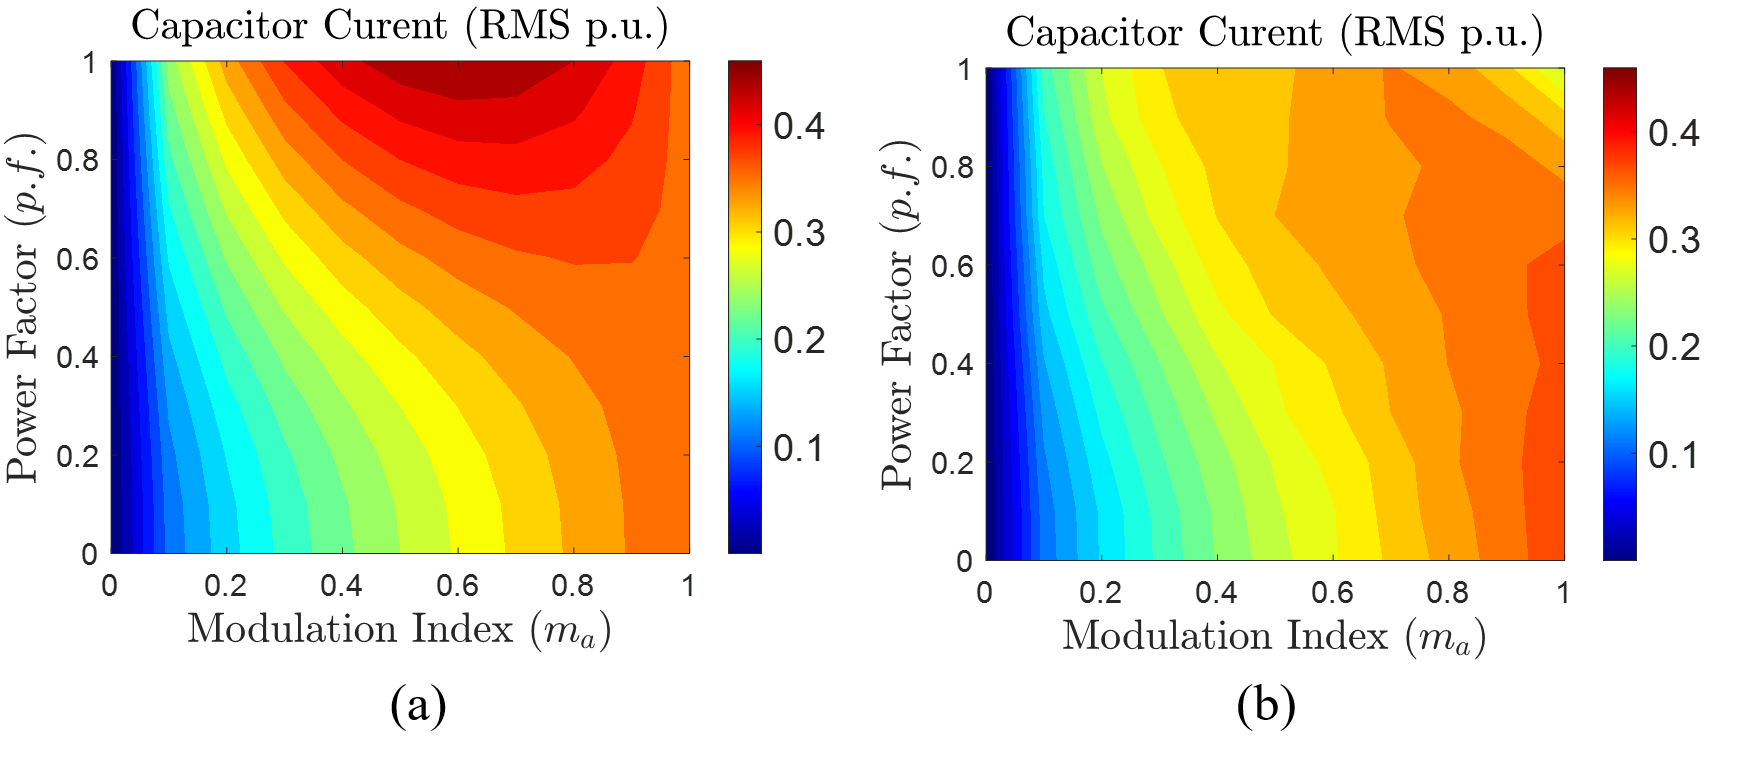
\includegraphics[width=1\linewidth]{A-Figures/Simulation/RMSComparisonTotal.png}
    \vspace{-8mm}
    \caption{RMS capacitor currentacross varying \( m_a \) and power factor values. a) The conventional single-carrier PWM. b) The proposed multicarrier PWM method }
    \label{fig:rms_results_tot}
\end{figure}


\color{red}
Remaining sections will be provided in the full paper. 
\section{Implementation Methodology}
% While the proposed adaptive multi-carrier PWM technique offers significant improvements in reducing DC-link capacitor current stress, direct real-time optimization of carrier phase shifts in each switching cycle is computationally prohibitive. To overcome this, an offline optimization and reduced-dimension lookup table (LUT)-based implementation strategy is developed to ensure real-time feasibility.

% The section will be provided in the full paper. 

% \subsection{Offline Optimization with Reduced-Dimension Inputs}

% In each switching cycle, the optimal carrier phase shifts \( (\theta_b^{opt}, \theta_c^{opt}) \) are determined by minimizing the capacitor current RMS over that switching interval. However, performing this optimization in real-time is not feasible due to the high dimensionality and computational cost. To address this, the following steps are adopted:

% \begin{itemize}
%     \item \textbf{Current normalization:} The instantaneous time-domain phase currents \( i_a(t), i_b(t), i_c(t) \) are normalized with respect to the sum of their absolute values:
%     \[
%     \hat{i}_x(t) = \frac{i_x(t)}{|i_a(t)| + |i_b(t)| + |i_c(t)|}, \quad x \in \{a, b, c\}
%     \]
%     This normalization provides scale-invariance and focuses the optimization on the relative distribution and direction of currents.
    
%     \item \textbf{Dimensionality reduction:} Since the three-phase system is inherently balanced (i.e., \( i_a + i_b + i_c = 0 \)), only two normalized current values are sufficient to describe the system. Hence, the input current space is reduced to:
%     \[
%     \{ \hat{i}_a, \hat{i}_b \}
%     \]
    
%     \item \textbf{Duty cycle reduction:} In sinusoidal PWM (SPWM), the duty cycles of the three legs satisfy the constraint \( d_a + d_b + d_c = \frac{3}{2} \), allowing any two duty cycles to fully define the modulation state. Thus, only \( d_a \) and \( d_b \) are required as LUT inputs.
% \end{itemize}

% Using this reduced set of variables, the offline optimization computes the optimal phase shifts \( (\theta_b^{opt}, \theta_c^{opt}) \) over a grid of operating conditions by minimizing the capacitor RMS current within the switching interval.



 
% \subsection{Lookup Table Construction}

% A four-dimensional lookup table is constructed where each entry maps the operating point defined by \( (\hat{i}_a, \hat{i}_b, d_a, d_b) \) to optimal phase shifts \( (\theta_b^{opt}, \theta_c^{opt}) \):
% \[
% \text{LUT} : (\hat{i}_a, \hat{i}_b, d_a, d_b) \mapsto (\theta_b^{opt}, \theta_c^{opt})
% \]
% The input space is uniformly sampled over practical ranges, and linear or bilinear interpolation is used to estimate values between stored points, ensuring continuity and smooth transition across operating conditions.

% \subsection{Real-Time Control Execution}

% During real-time operation, the control algorithm executes the following steps in each PWM cycle:

% \begin{enumerate}
%     \item Measure instantaneous phase currents \( i_a(t), i_b(t), i_c(t) \).
%     \item Normalize the currents to obtain \( \hat{i}_a \) and \( \hat{i}_b \).
%     \item Compute the duty cycles \( d_a \) and \( d_b \) from the voltage references.
%     \item Access the LUT using \( (\hat{i}_a, \hat{i}_b, d_a, d_b) \) to retrieve \( (\theta_b^{opt}, \theta_c^{opt}) \).
%     \item Apply the phase shifts to the carrier signals of legs B and C.
%     \item Generate PWM gate signals using standard SPWM comparison.
% \end{enumerate}

% % \subsection{Hardware and Memory Considerations}
% % The proposed method is implemented on a real-time control platform (Imperix B-Box RCP), which provides deterministic execution and high-speed memory access. The compact LUT is stored in on-chip memory, and the computational overhead of the lookup and interpolation remains negligible within the PWM cycle duration.

% \subsection{Benefits of the Approach}
% The proposed implementation strategy effectively bridges the gap between optimality and practicality.
% By leveraging current normalization and system symmetry, the input space is significantly reduced, allowing compact and efficient LUT construction. 
% This enables real-time execution without sacrificing the performance advantages of adaptive carrier phase shifting, making the technique suitable for industrial inverter applications with strict timing and reliability requirements.


% \section{Simulation Results}
%  The section will be provided in the full paper. 

\section{Experimental Validation}
 % The section will be provided in the full paper.
 
% To validate the effectiveness of the proposed multi-carrier PWM technique, a laboratory-scale experimental setup was established using a two-level three-phase inverter, connected to an induction machine, as given in Fig. \ref{fig:experimentalsetup}. 

% \begin{figure}[h!]
% \centering 
% 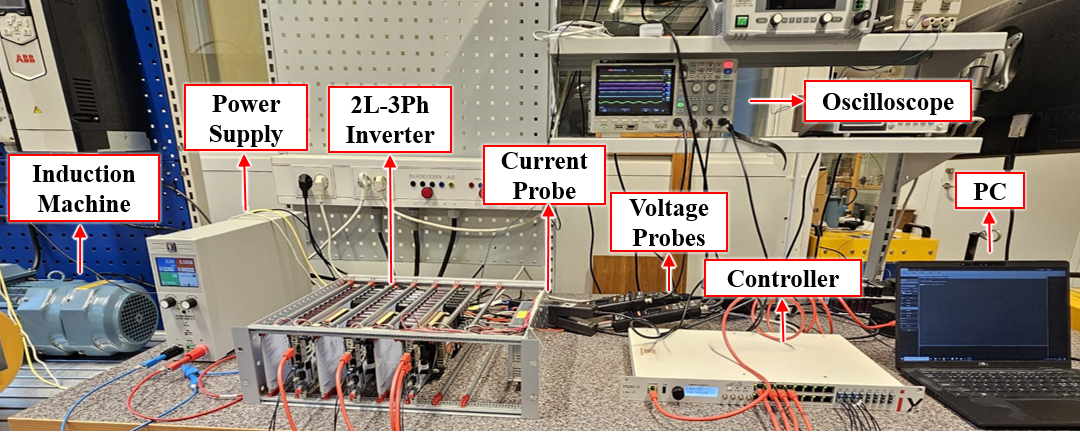
\includegraphics[width=1\linewidth]{A-Figures/ExperimentalSetupv2.png}  
% \caption{ a) The system structure of a conventional 2-level 3-phase inverter connected to an induction machine. }
%     \label{fig:experimentalsetup}
% \end{figure}

% The setup utilizes a real-time control platform (Imperix B-Box RCP) operating at a switching frequency of 10kHz, with gate signals generated according to both the conventional and proposed PWM schemes.

% Current sensors were placed at the DC-link to measure the instantaneous capacitor current, and the RMS values were computed using a high-resolution oscilloscope.

% Fig.~\ref{fig:experimental_waveforms} shows the measured DC-link current waveforms under induction machine load and a modulation index. 

% \begin{figure}[h!]
% \centering
% 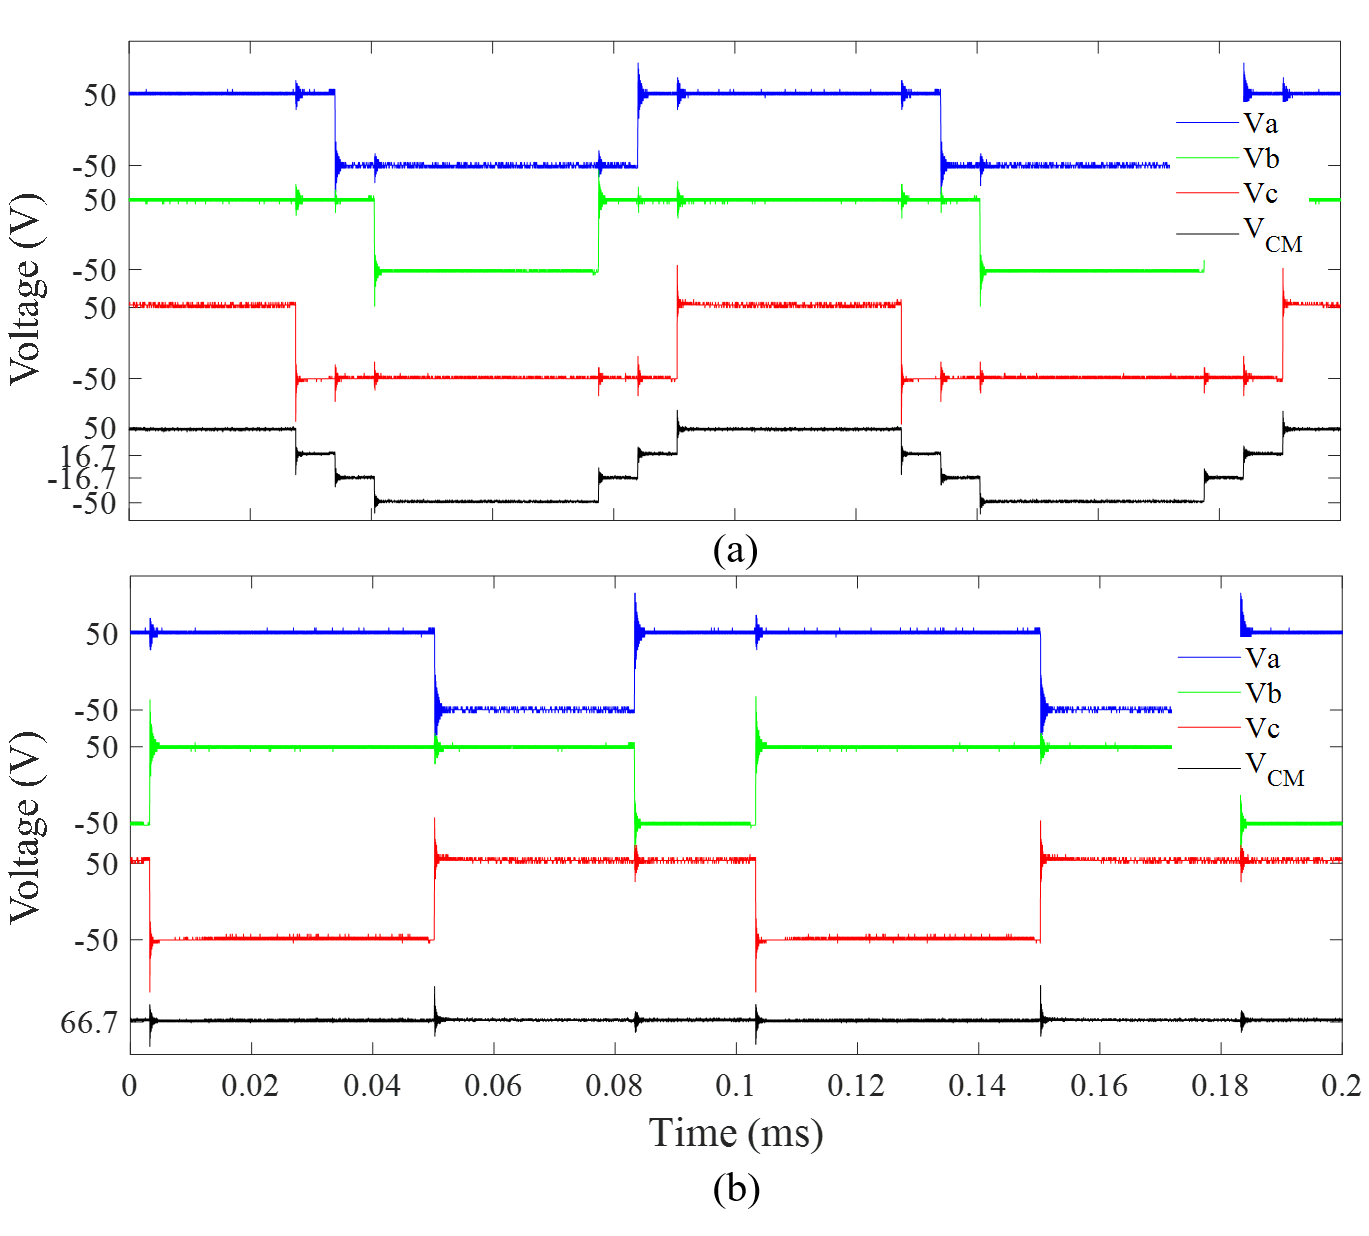
\includegraphics[width=1\linewidth]{A-Figures/noloadSinusModulationCloseup.png}
% \caption{Measured DC-link capacitor current: (a) Conventional PWM, (b) Proposed Multi-Carrier PWM.}
% \label{fig:experimental_waveforms}
% \end{figure}

% Additionally, Fig.~\ref{fig:experimental_rms} summarizes the RMS current values obtained from multiple operating points, confirming that the proposed method consistently reduces RMS current by 15–30\% across different operating conditions.

% \begin{figure}[h!]
% \centering
% 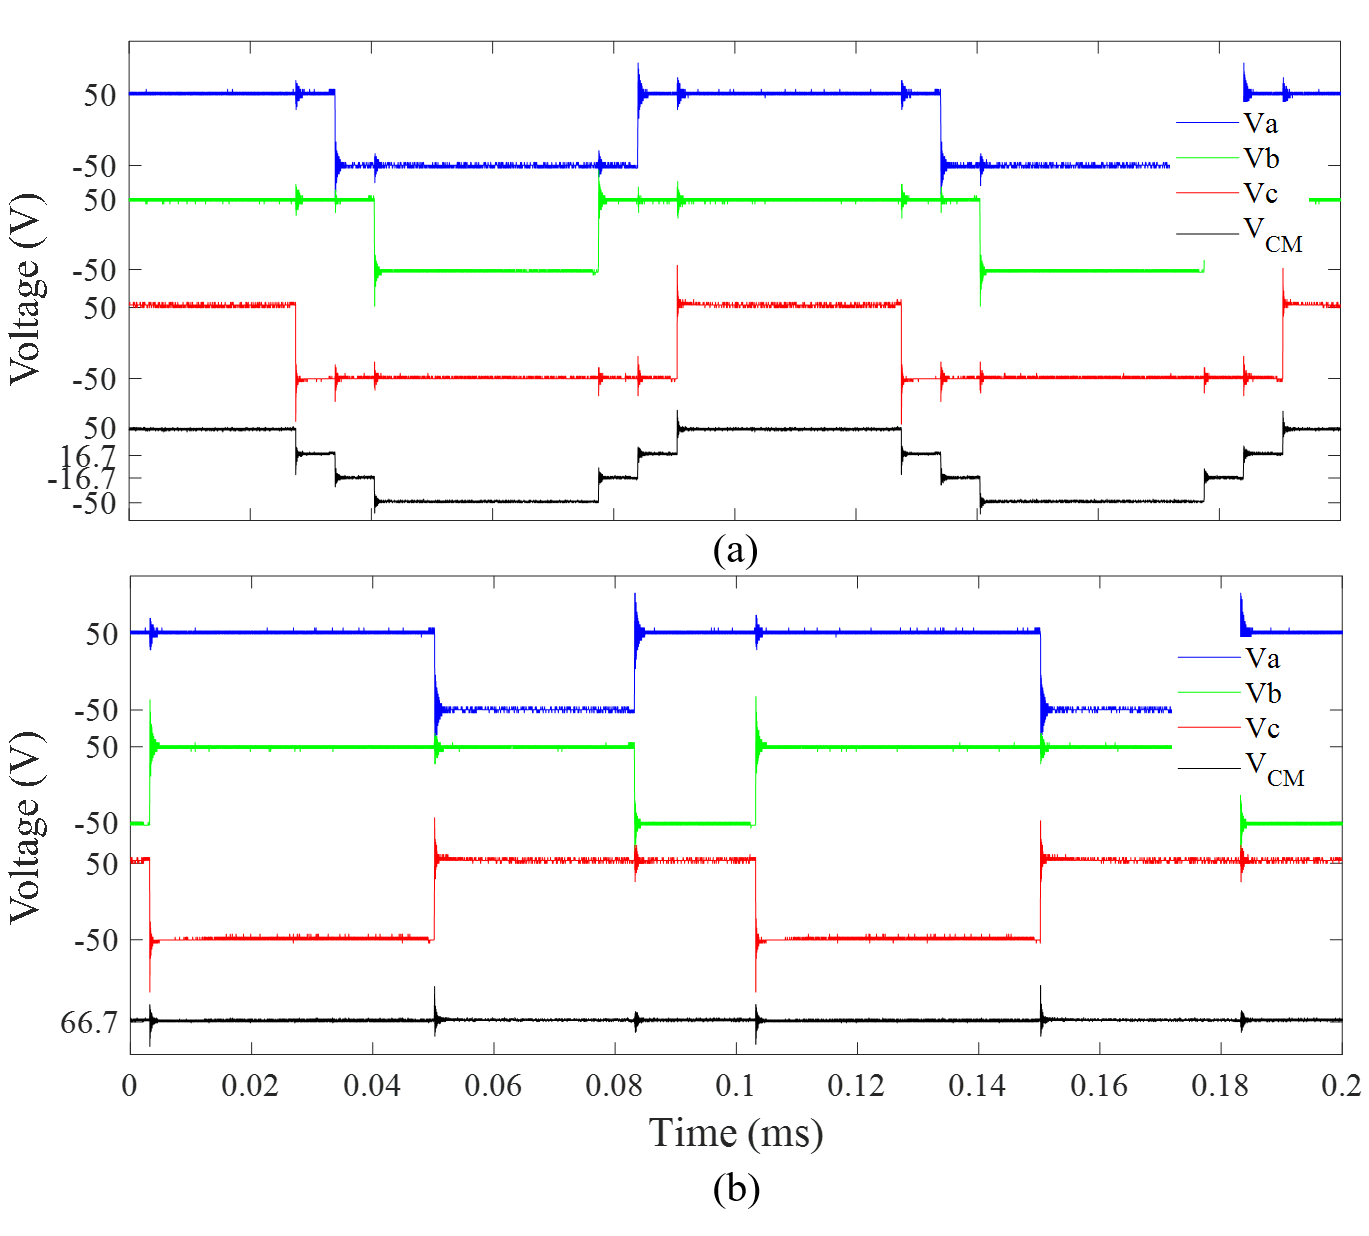
\includegraphics[width=1\linewidth]{A-Figures/noloadSinusModulationCloseup.png}
% \caption{Comparison of measured RMS DC-link current between conventional and proposed PWM methods.}
% \label{fig:experimental_rms}
% \end{figure}

% These experimental results validate the simulation findings and demonstrate the practical applicability of the proposed modulation strategy in reducing thermal stress and enhancing DC-link capacitor longevity.


\section{Conclusion and Future Work}
 % The section will be provided in the full paper.
% This paper introduces a novel multi-carrier PWM strategy for two-level three-phase inverters, which aims at reducing the current stress on DC-link capacitors. 
% Unlike conventional interleaving methods that require multiple inverter stages or hardware redundancy, the proposed technique dynamically adjusts the carrier phase shifts of each inverter leg based on real-time duty ratios and leg currents, enabling ripple minimization within a single inverter unit.
% To address the complexity of real-time optimization, the method exploits the symmetry of three-phase systems, allowing a reduced input space for a compact and efficient lookup table implementation. 
% Simulation results confirmed a consistent reduction in RMS capacitor current across a wide operating range, with improved thermal performance and extended capacitor lifetime.
% The proposed method was further validated experimentally on a laboratory setup using real-time digital control and high-resolution measurements. 
% The measured results confirmed that the proposed scheme achieved up to 30\% reduction in RMS capacitor current compared to conventional single-carrier PWM, verifying both the practicality and effectiveness of the strategy.
% Overall, the proposed technique offers a low-complexity, hardware-efficient solution for improving reliability and extending the lifetime of DC-link capacitors in industrial inverter applications. 

\color{black}

\bibliographystyle{IEEEtran}
\bibliography{Aref.bib}

\end{document}
